\begin{minipage}{0.4\linewidth}
\begin{figure}[H]
    \centering
    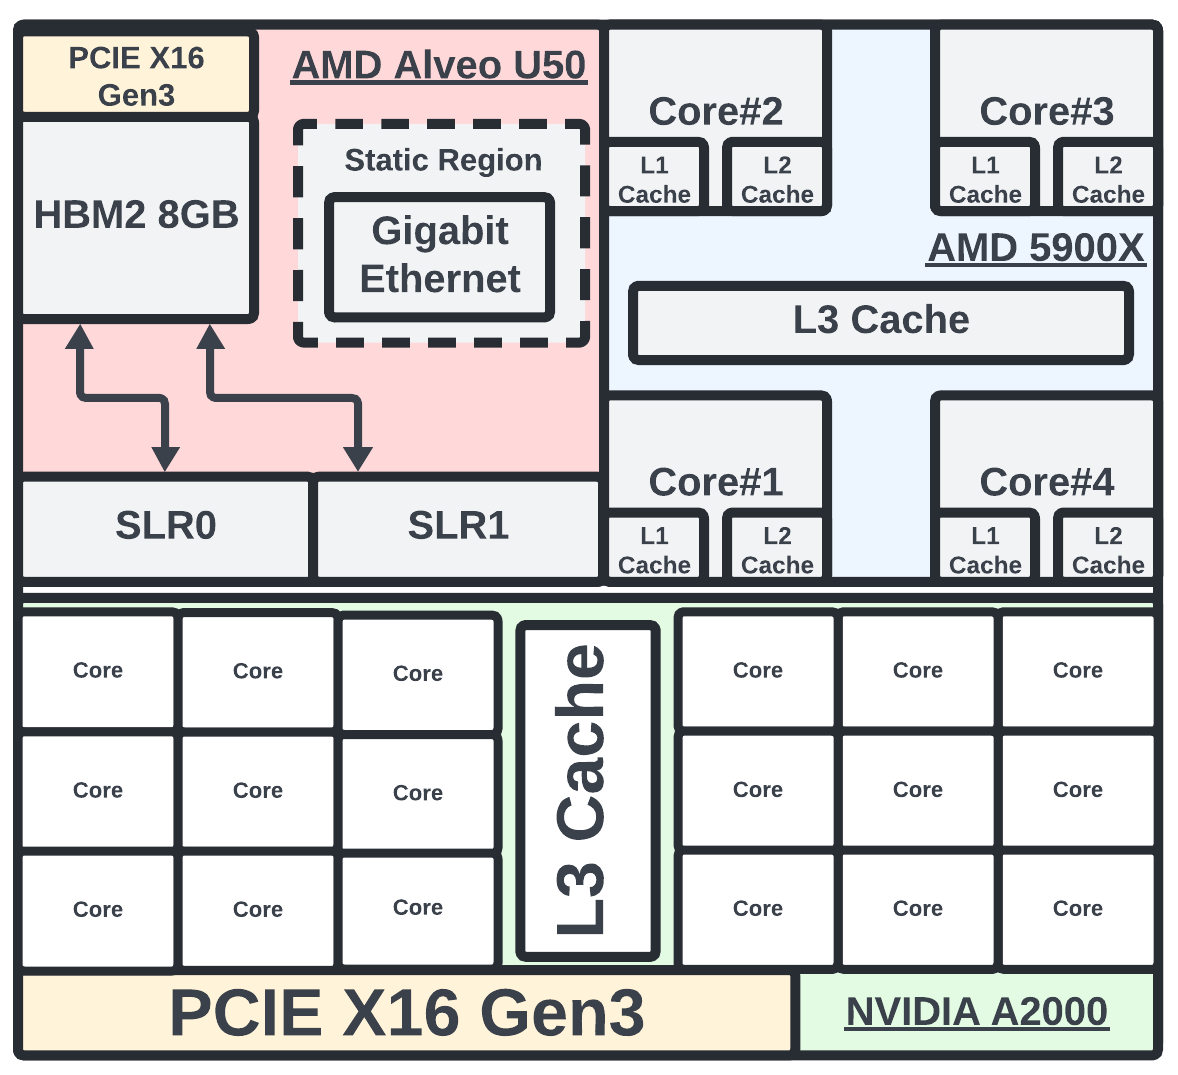
\includegraphics[width=\linewidth]{images/hardware.png} % Adjust the image width to fit the minipage
    \caption{Heterogeneous System Enviroment}
    \label{fig:HeterogenousHardware}
\end{figure}
\end{minipage}%
\hspace{5mm}
\begin{minipage}{0.6\linewidth}
\begin{table}[H]
\centering
\setlength{\extrarowheight}{0pt}
\addtolength{\extrarowheight}{\aboverulesep}
\addtolength{\extrarowheight}{\belowrulesep}
\setlength{\aboverulesep}{0pt}
\setlength{\belowrulesep}{0pt}
\caption{Hardware/Software Environment}
\label{tab:HWEnvironment}
\resizebox{\linewidth}{!}{%
\begin{tabular}{c|c|c|c} 
\toprule
\rowcolor[rgb]{0.753,0.753,0.753} \textbf{Accelerator} & \textbf{Hardware} & \begin{tabular}[c]{@{}>{\cellcolor[rgb]{0.753,0.753,0.753}}c@{}}\textbf{Language /}\\\textbf{Library}\end{tabular} & \multicolumn{1}{c|}{\begin{tabular}[c]{@{}>{\cellcolor[rgb]{0.753,0.753,0.753}}c@{}}\textbf{Energy}\\\textbf{Measurement}\end{tabular}} \\ 
\cmidrule{1-3}\cline{4-4}
CPU & \begin{tabular}[c]{@{}c@{}}AMD 5900x \\ (4.8 GHz)\end{tabular} & \begin{tabular}[c]{@{}c@{}}Python / \\Pytorch 2.4\end{tabular} & RAPL \\ 
\cmidrule{1-3}\cline{4-4}
GPU & \begin{tabular}[c]{@{}c@{}}Nvidia A2000 \\ (1200 MHz)\end{tabular} & \begin{tabular}[c]{@{}c@{}}Python / \\Pytorch 2.4\end{tabular} & Nvidia SMI \\ 
\cmidrule{1-3}\cline{4-4}
FPGA & \begin{tabular}[c]{@{}c@{}}U50 \\ (300 MHz)\end{tabular} & \begin{tabular}[c]{@{}c@{}}HLS (C++) / \\Vitis Vision\end{tabular} & Xbutil \\
\bottomrule
\end{tabular}
}
\end{table}
\end{minipage}
\newline